\documentclass[sigconf,edbt]{acmart-edbt-workshops}

\usepackage{booktabs} % For formal tables
\usepackage{hyperref}       % hyperlinks
\usepackage{url}            % simple URL typesetting
\usepackage{booktabs}       % professional-quality tables
\usepackage{amsfonts}       % blackboard math symbols
\usepackage{nicefrac}       % compact symbols for 1/2, etc.
\usepackage{microtype}      % microtypography
\usepackage{cleveref}
\usepackage{amsmath,amssymb}             % AMS Math
\usepackage{dsfont}
\usepackage{mathtools}

\usepackage{algorithm}
\usepackage{algpseudocode}

\usepackage{tikz}

\usepackage{array}
\usepackage{multirow}

\usetikzlibrary{shapes,backgrounds, calc, shadings, arrows,decorations.pathmorphing,backgrounds,fit,positioning,shapes.symbols,chains}
\pgfdeclareradialshading{ballshading}{
 \pgfpoint{-10bp}{10bp}}
 {color(0bp)=(gray!50!black);
  color(9bp)=(gray!50!black);
  color(18bp)=(gray!50!black);
  color(25bp)=(gray!50!black);
  color(50bp)=(black)}

\tikzstyle{peers}=[draw,circle, minimum width=10pt]
\tikzstyle{superpeers}=[draw,circle,minimum width=20pt]

\tikzset{
%Define standard arrow tip
>=stealth',
%Define style for different line styles
help lines/.style={dashed, thick},
axis/.style={<->},
important line/.style={thick},
connection/.style={thick, dotted},
}
\newcommand\A{\ensuremath{\mathcal{A}}}
\newcommand\B{\ensuremath{\mathcal{B}}}

\newcommand\cmbox[1]{
  \fbox{\lower0.75cm
    \vbox to 1.0cm{\vfil
      \hbox to 1.7cm{\hfil\parbox{1.4cm}{\centering #1}\hfil}
      \vfil}%
  }%
}

\newcommand\cmlegend[1]{
  {\lower0.75cm
    \vbox to 1.0cm{\vfil
      \hbox to 0.7cm{\hfil #1}
      \vfil}%
  }%
}

% Copyright
\setcopyright{rightsretained}

% DOI
\acmDOI{}

% ISBN
\acmISBN{978-3-89318-078-3}

%Conference
\acmConference[EDBT 2018]{21st International Conference on Extending Database Technology (EDBT)}{March 26-29, 2018}{Vienna, Austria} 
\acmYear{2018}

\settopmatter{printacmref=false, printccs=false, printfolios=false}

\pagestyle{plain} % removes running headers

\def\HCBR{{\sc HCBR}}
\def\bfHCBR{{\sc \bf HCBR}}

\newcommand{\mynote}[1]{{\bf  \textcolor{blue}{#1}}}
\begin{document}
\title{Binary Classification With Hypergraph Case-Based Reasoning}
%\titlenote{Produces the permission block, and copyright information}
%\subtitle{Extended Abstract}
%\subtitlenote{The full version of the author's guide is available as
%  \texttt{acmart.pdf} document}
  

\author{Alexandre Quemy} 
\affiliation{%
 \institution{IBM Software Lab}
 \city{Cracow} 
 \country{Poland}}
\affiliation{%
  \institution{Faculty of Computing, Pozna\'n University of Technology}
  \city{Pozna\'n} 
  \country{Poland}
}
\email{aquemy@pl.ibm.com}


% The default list of authors is too long for headers}
% \renewcommand{\shortauthors}{B. Trovato et al.}
\renewcommand{\shortauthors}{}


\begin{abstract}
Binary classification is one of the most common problem in machine learning. It consists in predicting whether a given element is of a particular class. In this paper, a new algorithm for binary classification is proposed using a hypergraph representation. Each element to be classified is partitioned according to its interactions with the training set. For each class, the total support is calculated as a convex combination of the {\it evidence} strength of the element of the partition. The evidence measure is pre-computed using the hypergraph induced by the training set and iteratively adjusted through a training phase. It does not require structured information, each case being represented by a set of {\it agnostic information} atoms. Empirical validation demonstrates its high potential on a wide range of well-known datasets and the results are compared to the literature. The time complexity is given and empirically validated. Its capacity to provide good accuracy with few examples is also studied.
\end{abstract}

\maketitle



%%%%%%%%%%%%%%%%%%%%%%%%%%%%%%%%%%%%%%%%%%%%%%%%%%%%%%%%%%%%%%%%%%%%%%%%%%%%%%%
\section{Introduction}\label{sec:intro}
%%%%%%%%%%%%%%%%%%%%%%%%%%%%%%%%%%%%%%%%%%%%%%%%%%%%%%%%%%%%%%%%%%%%%%%%%%%%%%%

In many real-life situations, one tries to take a decision based on previous {\it similar} situations. Each situation is described by a certain amount of information, either collected by an expert according to the relevance of the information, or automatically by some sensors or algorithms. Those situations share similarities on which to make analogies or counter-examples in order to take a new decision. Conversely, in general, if two situations do not share any common characteristic, then they are totally independent, i.e. it is impossible to infer one's outcome from the other one. The purpose of supervised machine learning algorithms is to exploit the available information and interactions between past cases or examples in order to build a model or infer the key rules to take correct decisions.

Due to the large variety of concrete situations that can be reduced to binary classification, it is one of the most studied problems in machine learning. In this paper, we investigate the problem of binary prediction under a supervised setting, i.e. given a history of previous situations labeled with the correct output.

This paper contributes to binary classification with a new algorithm called Hypergraph Case-Based Reasoning (\HCBR). The idea is to create a hypergraph where each element of the training set is a hyperedge and vertices are represented by the features describing the elements. The intersections between edges create a partition for each case, and we model the support for each class as a convex combination of the elements of this partition. Each of those elements is valued according to its importance w.r.t. to the set of all the hyperedges it belongs to and their respective labels.

The well-known "no free lunch" theorem states that there is no unique algorithm that can outperform all the others in supervised learning. However, the case description and representation play a preponderant role in the performances but the algorithms are very often constrained by being designed to a specific representation that may not be suitable for a given problem or user data. The proposed method is totally agnostic about the representation\footnote{With the exception that the current version must work on discrete information.} and does not require structured representations. For instance, it can work on atomic representations such as Bag-of-Word representations for texts where an atom is a single word (or $n$-gram). In this case, two elements would not have the same number of elements and it may be hard to properly define the case domain.

The plan of the paper is as follows: in Section \ref{sec:problem} the problem of binary classification is formalized in the particular case of a finite countable set of information. The contribution of this paper is divided into two parts: Section \ref{sec:model} defines the \HCBR~ algorithm and Section \ref{sec:experiments} presents empirical results on 8 datasets from the UC Irvine Machine Learning Repository (UCI)\footnote{\href{http://archive.ics.uci.edu/ml/index.php}{http://archive.ics.uci.edu/ml/index.php}} and the LIBSVM\footnote{\href{https://www.csie.ntu.edu.tw/~cjlin/libsvmtools/datasets/binary.html}{https://www.csie.ntu.edu.tw/~cjlin/libsvmtools/datasets/binary.html}}. The paper ends in Section \ref{sec:conclusion} with a discussion about the results, future work, and possible improvements.

\section{Classification and Hypergraph}
\label{sec:state_of_art}

Hypergraphs generalize graphs and can be used to represent higher order relations while graphs are limited to binary relations. A hypergraph is defined by a set of vertices and a collection of hyperedges where each hyperedge is a subset of this set of vertices. Therefore, a graph is a special case of hypergraph for which each hyperedge contains only two vertices. We will formally introduce hypergraphs in Section \ref{sec:rep}.
Recently hypergraphs have been used as data representation, and some classification algorithms on hypergraph have been proposed. A vast majority of approaches models the objects to classify as the set of vertices and constructs the hyperedges as the representation of a metric. This conventional approach is known as {\it neighborhood-based} hypergraph. The metric relies on some assumptions on the data or a specific representation (e.g. Zernike moment and histogram of oriented gradient (HOG) to measure the distance between images in \cite{ijcai2017-387}) and for each vertex, a hyperedge is created to represent its $k$-nearest neighbors \cite{5540012}. The problem of classification on hypergraph consists in labeling some unlabeled vertices given a training set such that all vertices in a same hyperedge have the same label. As all the vertices are known a priori, the problem is part of transductive learning. To learn the labels, the standard approach is to minimize a cost function based on a hypergraph equivalent of a graph Laplacian \cite{NIPS2006_3128,ijcai2017-387} with a structural risk:
\begin{align}
C(x) = x^t \Delta x + \mu ||x - y||^2
\end{align} where $\Delta$ is the hypergraph Laplacian, $\mu >0$ a regularization factor and $||.||$ a norm. The vector $y$ represents the initial labels for all vertices with $y_i = 0$ for unlabeled vertices, a negative (resp. positive) value for label -1 or 1.

On the contrary, the method proposed in this paper models the elements to classify as the hyperedges and the vertices as the different components of those elements. As far as we know, there is no previous work that uses this modeling choice. In addition, it does not require knowing all the elements before building the model: our approach is inductive. If the literature focus on the method to build the hyperedges, the proposed framework has a straightforward hypergraph construction and rather focus on model selection.

\section{Problem definition}
\label{sec:problem}

Consider a countable finite space of information $\mathbb{F}$ and its $\sigma$-algebra $\mathcal P({\mathbb F})$ defined as the powerset of $\mathbb F$. We call {\it case} an element of $\mathcal P({\mathbb F})$. In practice, it is very likely that only a subset of $\mathcal P({\mathbb F})$ may appear (for instance if two features encode two contradictory propositions or if every case has the same number of features). The real class for any case is defined by the unknown measurable mapping:
\begin{align*}
   J \colon \mathcal P({\mathbb F}) & \to \{0,1 \} \\
   x &\mapsto J(x)
\end{align*}

Given an example set $X$ of $n$ cases, the classification problem consists in minimizing the prediction errors for all the elements of $\mathcal P({\mathbb F})$, that is to say finding a decision mapping $\bar J \colon \mathcal P({\mathbb F}) \to \{0,1 \}$ such that:
\begin{align}
\label{eq:pb} 
 \forall X \in \mathcal P({\mathbb F})^n, ~ \underset{\bar J}{\min} \sum_{x \in \mathcal P({\mathbb F})} \mathds{1}_{\{J(x) \neq \bar J(x)\}}
\end{align}
In other words, for any possible training set, we want to find an estimation of the exact mapping $J$ and thus it is a functional problem.
Notice that in this paper we do not consider {\it uncertainty}: if two situations are described the same in $\mathbb{F}$, then they have the same label.

\section{Hypergraph Case-Based Reasoning}
\label{sec:model}

\subsection{Representation And Projection}
\label{sec:rep}

Before describing \HCBR, we recall the definition of a hypergraph and induced hypergraph. For more results on hypergraphs, we refer the reader to \cite{berge1984hypergraphs}.
\begin{definition}[Hypergraph]
A hypergraph is defined by $H = (V, X)$ with $V$ a set of vertices, $X$ the hyperedges such that $\forall x \in X, ~ x \subseteq V$.
\end{definition}
\noindent
A hypergraph can be viewed as a collection of subsets $X$ of a given set of vertices $V$. It is sometimes convenient to define a hypergraph solely by a collection of sets. In this case, the set of vertices, denoted $V_X$, is implicitly defined as the union of edges.

\begin{definition}[Induced Subhypergraph]
The subhypergraph $H[A]$ induced by $A \subseteq V$ is defined by $H[A] = (A, X_A)$ with $X_A = \{ x \cap A ~ | ~ x \cap A \neq \emptyset\}$.
\end{definition}
\begin{figure}[!h]
  \centering
  \def\firstcircle{(0,0) ellipse (1.5cm and 1cm)}
  \def\secondcircle{(80:-1cm) ellipse (1.5cm and 1cm)}
  \def\thirdcircle{(0:2cm) ellipse (1.5cm and 1cm)}
  \begin{tikzpicture}[scale=0.5, every node/.style={scale=1}]
      \begin{scope}[fill opacity=0.3]
          \filldraw[fill=gray, xscale=1.4, yscale=1.4] (-0.0,-0.0) plot [smooth cycle,tension=0.7, shift={(-4,-3.2)}] coordinates {(3,1) (5,1.2) (7,1) (8,3) (7,4.5) (5,4.5) (2,4) (1.7,2.5)};
          %\filldraw[fill=gray] (-3.5,-3.5) rectangle (4,2);
          \fill[red, rotate=30, xscale=1.4, yscale=1.4] \firstcircle;
          \fill[green, rotate=35, xscale=1.4, yscale=1.4] \secondcircle;
          \fill[blue, xscale=1.4, yscale=1.4] \thirdcircle;
          \draw[rotate=30, xscale=1.4, yscale=1.4] \firstcircle;
          \draw[rotate=35, xscale=1.4, yscale=1.4] \secondcircle;
          \draw[xscale=1.4, yscale=1.4] \thirdcircle;

      \end{scope}
      \node at (4,-2.7) {$\mathbb{F}$};
      \node at (0.5,1) {$x_1$};
      \node at (0,-2.3) {$x_2$};
      \node at (3,1) {$x_3$};

      \node at (-0.8  ,0.5) {$e_1$};
      \node at (1.4  ,0.7) {$e_2$};
      \node at (1.2  ,-0.3) {$e_3$};
      \node at (3.6  , -0.1) {$e_4$};
      \node at (2  , -0.7) {$e_5$};
      \node at (-0.4  ,-1) {$e_6$};
      \node at (1  ,-1.7) {$e_7$};
  \end{tikzpicture}
  \caption{\label{case_base} The family $\mathcal E = \{ e_i \}_{i}$ forms the partition obtained by the union of the projection of cases and represents how the three cases share information.}
\end{figure}

A set of examples $X$ can be seen as a hypergraph $H = (\mathbb F, X)$, i.e. such that each example is a hyperedge (Figure \ref{case_base}). In practice, we do not need to know $\mathbb{F}$ as we can always use the implicit hypergraph $H = (\mathbb{F}_X, X)$ where $\mathbb{F}_X$ is the restriction of $\mathbb{F}$ to the features that appear in the sample $X$.
\begin{definition}[Projection defined by a subhypergraph]
The projection operator $\pi_H$ over a hypergraph $H = (V, X)$ for any $A \subseteq V$ is defined by $\pi_H(A) = \{ e \subseteq A ~ | ~ \exists X' \subseteq X_A, ~ e = \underset{x \in X'}{\bigcap} x \}$.
\end{definition}
For a case $x$, the operator $\pi$ takes the subhypergraph $H[x]$ and returns the partition of the features of $x$ defined by the intersection family induced by $H[x]$. Each element of $\pi_H(x)$ is a (sub)set of features. For instance, in Figure \ref{case_base}, $\pi_H(x_1) = \{ e_1, e_2, e_3, e_6 \}$ and in Figure \ref{new_case_schema}, the projection of $x$ (in yellow) on $H$ is represented by the family $\{ e'_i\}_i$.
For convenience, for a given $H = (V_X, X)$, we denote by $\mathcal{E}_H = \{e_i\}^m_{i=1} = \{ e \in \underset{x \in X}{\cup} \pi_H(x)\}$ that is to say, the partition of $V_X$ obtained by the intersection of the edges. This partition is unique to a hypergraph.

We call {\it discretionary features} of $x$ (w.r.t. $H$) the set (possibly empty) of features that are not in any element of the projection $\pi_H(x)$, denoted $D_x$. It can be interpreted as the features of $x$ that do not belong to any hyperedge. If a hypergraph induced by a set of examples represents a knowledge base at a given moment, the discretionary features of $x$ are new pieces of information that were never encountered before. For instance, considering the hypergraph composed of $x_1$ and $x_2$ as illustrated by Figure \ref{case_base}, the set of discretionary features of $x_3$ is $e_4$. In Figure \ref{new_case_schema}, the yellow case $x$ has no discretionary feature: all its features are present at least in one example.

\begin{figure}[b]
  \def\firstcircle{(0,0) ellipse (1.5cm and 1cm)}
  \def\secondcircle{(80:-1cm) ellipse (1.5cm and 1cm)}
  \def\thirdcircle{(0:2cm) ellipse (1.5cm and 1cm)}
  \begin{tikzpicture}[scale=0.5, every node/.style={scale=0.7}]
      \begin{scope}[fill opacity=0.3]
          \filldraw[fill=gray, xscale=1.4, yscale=1.4] (-3.5,-3.5) plot [smooth cycle,tension=0.7, shift={(-4,-3.2)}] coordinates {(3,1) (5,1.2) (7,1) (8,3) (7,4.5) (5,4.5) (2,4) (1.7,2.5)};
          %\filldraw[fill=gray] (-3.5,-3.5) rectangle (4,2);
          \fill[red, rotate=30, xscale=1.4, yscale=1.4] \firstcircle;
          \fill[green, rotate=35, xscale=1.4, yscale=1.4] \secondcircle;
          \fill[blue, xscale=1.4, yscale=1.4] \thirdcircle;
          \draw[rotate=30, xscale=1.4, yscale=1.4] \firstcircle;
          \draw[rotate=35, xscale=1.4, yscale=1.4] \secondcircle;
          \draw[xscale=1.4, yscale=1.4] \thirdcircle;

          \fill[yellow, rotate=110, xscale=1, yscale=1, xshift=-10, yshift=15] \secondcircle;
          \draw[rotate=110, xscale=1, yscale=1, xshift=-10, yshift=15] \secondcircle;

      \end{scope}
      \node at (4,-2.7) {$\mathbb{F}$};
      \node at (0.5,1.3) {$x_1$};
      \node at (0,-2.3) {$x_2$};
      \node at (3,1) {$x_3$};

      \node at (-0.8  ,0.5) {$e_1$};
      \node at (0.2  ,0.6) {$e_1'$};
      \node at (1.5  ,0.7) {$e_2$};
      \node at (1.05  ,0.5) {$e_2'$};
      \node at (1.2  ,-0.2) {$e_3'$};
      \node at (1.675  , 0.15) {$e_3$};
      \node at (3.6  , -0.1) {$e_4$};
      \node at (2  , -0.7) {$e_5$};
      \node at (1.5 , -0.8) {$e_5'$};
      \node at (-0.6  ,-1.2) {$e_6$};
      \node at (0.3  ,-0.7) {$e_6'$};
      \node at (1  ,-1.4) {$e_7'$};
      \node at (0.5  ,-2) {$e_7$};
  \end{tikzpicture}
  \begin{tikzpicture}[auto, thick, scale=0.6, every node/.style={scale=0.8}, baseline={(-2,-0)}]
    % Place super peers and connect them
    \node[superpeers, fill=red!30] (c1) at  (0,-4) {$x_1$};
    \node[superpeers, fill=blue!30] (c2) at  (2,-4) {$x_2$};
    \node[superpeers, fill=green!30] (c3) at  (-2,-4) {$x_3$};
    \node[superpeers, fill=yellow!30] (c4) at (0,0) {$x$};
    %\foreach \source/\dest in {a/b, a/c, a/d, b/c, c/d,a/e,d/e}
    %  \path (\source) edge (\dest);
     \node[peers, fill=black!10, label=above:{$e_2'$}] (e2) at (-2.5,-2) {};
     \node[peers, fill=black!10, label={[xshift=0.05cm, yshift=-0.05cm]{$e_3'$}}] (e3) at (-1.5,-2) {};
     \node[peers, fill=black!10, label={[xshift=-0.1cm, yshift=-0.05cm]{$e_5'$}}] (e5) at (-0.5,-2) {};
     \node[peers, fill=black!10, label={[xshift=0.1cm, yshift=-0.1cm]{$e_1'$}}] (e1) at (0.5,-2) {};
     \node[peers, fill=black!10, label={[xshift=-0.1cm, yshift=-0.1cm]{$e_6'$}}] (e6) at (1.5,-2) {};
     \node[peers, fill=black!10, label=above:{$e_7'$}] (e7) at (2.5, -2) {};


     \path[<-] (c4) edge (e1);
     \path[<-] (c4) edge (e2);
     \path[<-] (c4) edge (e3);
     \path[<-] (c4) edge (e5);
     \path[<-] (c4) edge (e6);
     \path[<-] (c4) edge (e7);

     \path[->] (c1) edge (e1);
     \path[->] (c1) edge (e2);
     \path[->] (c1) edge (e3);
     \path[->] (c1) edge (e6);

     \path[->] (c2) edge (e3);
     \path[->] (c2) edge (e5);
     \path[->] (c2) edge (e6);
     \path[->] (c2) edge (e7);

     \path[->] (c3) edge (e2);
     \path[->] (c3) edge (e3);
     \path[->] (c3) edge (e5);

  \end{tikzpicture}
  \caption{\label{new_case_schema} The projection of $x$ on $H$ is represented by the family  $\{ e'_i\}_i$. Under the projection lies a graph representation of $x$ with the partition elements $\{ e_i\}_i$ and their respective connections to the cases $\{x_i\}_i$, in particular, $D_x = \emptyset$.}
\end{figure}

For any set of features $x \subseteq \mathbb F$, we define $d_H(x) = \{ x' \in X ~ | ~ x \cap x' \neq \emptyset \}$ the set of edges sharing some features with $x$. In particular, the set $d_H$ can be split into $d_H^{(1)}$ and $d_H^{(0)}$ depending on the label of the case and defined by $d_H^{(l)}(x) = \{x' \in d_H(x) ~ | ~ J(x') = l \}$. $|d_H(x)|$ corresponds to the number of cases the case $x$ intersects while $|d_H^{(l)}(x)|$ counts the number of times the class $l$ is used among this set of intersecting cases. Note that if $x \not \in X$ and $|d_H(x)| = 0$, then $x = D_x$, i.e. the case $x$ is in relation with no case in $X$. In the hypergraph literature, $|d(x)|$ is called the {\it degree} of a hyperedge and its domain of definition is restricted to $X$.

From now, we consider only the specific hypergraph generated by the set of examples $X$. For the sake of readability, we remove the subscript $H$.

\subsection{Model Space}

In many binary classification approaches such as SVM or logistic regression, the model space consists of the set of hyperplanes of a given inner product space, usually $\mathbb{R}^M$. A hyperplane in $\mathbb{R}^M$ is uniquely defined by $M+1$ parameters. For an input vector $x$, its margin $m(w,x)$ is defined by its distance to a hyperplan defined by $w$ and is negative in case $x$ is wrongly classified, positive otherwise. Thus, the problem consists in finding the {\it best} parametrization to minimize a loss function summed over the training set. For instance, the Perceptron algorithm minimizes the 0-1 loss, SVM the hinge loss, and the Logistic Regression uses the log loss. Those functions are defined by \eqref{eqn:loss_functions}.
\begin{align}
  \label{eqn:loss_functions}
  \begin{matrix}
    L_{01}({w}, {x}) & = & \mathds{1}_{\{ m({w}, {x}) \leq 0 \}} \hfill \\
    L_{\text{hinge}}({w}, {x}) & = & \max(0, 1 - m({w}, {x})) \hfill \\
    L_{\log}({w}, {x}) & = & \ln(1 + e^{- m{w}, {x})}) \hfill
  \end{matrix}
\end{align}

In this paper, we relax the three implicit constraints on the input vector space:
\begin{enumerate}
\item we do not assume to have any inner product or metric embedded with the input vector space,
\item we do not assume the cardinality of the input vectors, such that it is possible to build a model and make predictions on incomplete systems (for instance missing in some rows in a database or Bag-of-Words representation),
\item we do not assume anything about the concrete {\it representation} of features while in most classification methods, all the features belongs to the same space, often $\mathbb{R}$.
\end{enumerate}
As a counterpart, \HCBR~ relies on two assumptions: (i) the correct class of an input vector is the result of its features only and (ii) if two input vectors $x$ and $x'$ do not share any feature, they are {\it independent} i.e. $x$ cannot help to understand the correct class of $x'$ and vice versa. As a result, \HCBR~  produces only {\it local} models because if a new input vector is independent of all examples, it is impossible to generate a prediction. On the contrary, a hyperplane model is {\it global} in a sense that it can produce a prediction for any element of $\mathbb{R}^M$.
A concrete situation for which such assumptions are natural is a justice trial. Cases are composed of some elements, and the correct label is the result of a reasoning that can possibly use analogies or counter-examples with a set of past cases on top of the legal texts. However, if a judge or lawyer wants to use $x$ to justify the outcome of $x'$, $x'$ must have similarities with $x$.

Let us formally define the model space. Given the hypergraph $H = (\mathbb F, X)$ defined by a training set $X$ and its associated partition $\mathcal{E} = \{e_i\}_i^m$, the relation between an example $x$ and its class is modeled by
\begin{align}
\label{eqn:model}
\left\{\begin{matrix}
s_{w, \mu}({x}) & = & \underset{i = 1}{\overset{m}\sum} w({e}_i, {x}) \mu({e}_i)% = <\mathbf{w}_i, \mathbf{\mu}_i >_{( \mathbf{X}, \mathbf{y})}
\\
\underset{i = 1}{\overset{m}\sum} w({e}_i,{x}_j) & = & 1 ~ \hfill \forall 1 \leq i \leq n\\
\underset{i = 1}{\overset{n}\sum} \mu({e}_i) & = & 1 \hfill \forall 1 \leq i \leq m \hfill
\end{matrix}\right.
\end{align} where $w({e}_i, {x}_j) \geq 0$ models the importance of ${e}_i$ in ${x}_j$ and $\mu({e}_i)$ the support of ${e}_i$ for class 1 w.r.t. whole training set. For this reason, we call $\mu$ the {\it intrinsic strength} of $e_i$. The assumption (ii) implies that if ${e}_i \cap {x}$ then $w({e}_i, {x}) = 0$. For readability, we write $s$ in place of $s_{w, \mu}$.

The classification rule consists in selecting the class with the total highest support.
 \begin{align} \tag{R1} \label{eqn:decision_rule}
 \forall x \in \mathcal{P}(\mathbb F), ~ 
   \bar J(x) =  \left\{\begin{matrix}
  1 & ~s(x) > 0\\ 
  0 & ~s(x) \leq  0
  \end{matrix}\right.
  \end{align} Our goal is to select $w$ and $\mu$ such that the classification rule \eqref{eqn:decision_rule} provides a good solution to the original problem \eqref{eq:pb}. For this purpose, we proceed in three steps:

  \begin{enumerate}
  \item Define $w$ and $\mu$ to capture as much information as possible from $\mathcal E$ for any $X$ (Section \ref{sec:model_selection}).
  \item Train the model to adjust the intrinsic strength on a specific $X$ using the classification rule \eqref{eqn:decision_rule} (Section \ref{sec:decision_training}).
  \item Refine the classification rule \eqref{eqn:decision_rule} to take into account the local nature of the model (Section \ref{sec:decision_training}).
  \end{enumerate} A summary and high level view of \HCBR~ is given by Algorithm~\ref{algo:HCBR}.

\algrenewcommand\algorithmicindent{1.0em}%
\begin{algorithm}
  \caption{HCBR (High level view)}\label{algo:HCBR}
  \begin{algorithmic}[1]
    \State Build $H$ and $\mathcal E$ from $X$.
    \State Calculate $w$ and $\mu$ on $\mathcal E$.
    \State Adjust $\mu$ with training algorithm \ref{training} on $X$ using rule \eqref{eqn:decision_rule}
    \For{each $x$ in test set}
        \State Calculate the projection $\pi(x)$.
        \State Calculate the support $s(x)$ using the projection.
        \State Predict using the updated rule \eqref{eqn:updated_cr}.
    \EndFor
  \end{algorithmic}
\end{algorithm}


While SVM aims at separating the data using a single hyperplane in the original input vector space, \HCBR~ tries to explain the decision for each case by a convex combination expressed in a lower dimensional space $\mathcal E$ generated by the data. In addition, the convex combinations depend on each other since the elements of $\mathcal E$ are by definition the features resulting in the case intersections. For any case, the decision rule is a combination of the strength of the elements of its projection on the hypergraph.

\subsection{Model Selection}
\label{sec:model_selection}

In this section, we define how to concretely select and calculate $w$ and $\mu$ for a given hypergraph. To ease the notation and for practical reasons, the measure $\mu$ is provided w.r.t. the intersection family $\mathcal E$ of the hypergraph induced by the training set $X$. However, $\mu$ can be defined over any partition of $\mathbb F$.

For $x$ and $x'$ in $\mathcal P({\mathbb F})$, a basic quantitative measure on the importance of $x'$ w.r.t. $x$ can be expressed by $\frac{|x \cap x'|}{|x|}$, i.e. how much $x'$ overlaps with $x$. This measure is a sort of {\it potential} for an analogy with $x$. Potential because it does not account for the individual importance of the features and simply holds the idea that the larger is a subset of features in a case, the higher is the chance it holds important features to decide the outcome.

Let us consider $\mathcal E$ and an example $x \in X$.
\begin{definition}[Intrinsic strength w.r.t. $x$]
  The intrinsic strength of $e \in \mathcal E$ w.r.t. $x \in X$ is defined by \begin{align}
    \begin{split}
    \forall l \in \{ 0, 1\}, ~ S^{(l)}(e, x) & = \frac{|d^{(l)}(e)| \frac{|x \cap e|}{|x|}}{\underset{e_j \in \mathcal E}{\sum}|d^{(l)}(e_j)|  \frac{|x \cap e_j|}{|x|}} \\
    & = \frac{|d^{(l)}(e)|  |x \cap e|}{\underset{e_j \in \mathcal E}{\sum}|d^{(l)}(e_j)| |x \cap e_j|}
    \end{split}
    \end{align}
  %\mynote{Maybe it would be better to define it over any partition first.}
\end{definition}
\noindent
In particular, for a given $x \in X$, $S^{(l)}(e_i, x) =0$ if $e_i$ is not part of the projection of $x$ on $H$. Also, $\underset{e \in \mathcal E}{\sum} S^{(l)}(e, x) = 1$ which can be interpreted as how much $e$ accounts for the set of labels $l$ the element $x$ holds in its projection.
The more $e_i$ belongs to many cases with the same class $l$ and the higher $S^{(l)}(e_i, x)$ is. Conversely, for a fixed number of cases, the more $e_i$ describes $x$, the higher $S^{(l)}(e_i, x)$ is. As $\forall e_i \in \mathcal E, ~ |d(e_i)| > 0$, either we have $S^{(1)}(e_i, x) \neq 0$ or $S^{(0)}(e_i, x) \neq 0$. We have $S^{(l)}(e_i, x) = 0$ only when all the cases in which $e_i$ results of are labeled with the opposite class $\bar l$. For $S^{(l)}(e_i, x) = 1$, it needs both the unanimity of labels for the cases in which $e_i$ belongs to and that $e_i = x$. The relation $e_i = x$ implies that $x$ does not share any feature with any other examples or that $x$ is included into another example.
\begin{definition}[Intrinsic strength w.r.t. a hypergraph $H$]
  \label{intrinsic_strength}
  The instrinsic strength of $e \in \mathcal{E}$ w.r.t. $H = (\mathbb{F}_X, X)$ is defined by
  \begin{align}
  \begin{split}
  \forall l \in \{ 1, 0 \}, ~ S^{(l)}(e) & = \frac{|e|}{ \underset{e' \in \mathcal{E}}{\sum} |e'|} \underset{x \in d^{(l)}(e)}{\sum} S^{(l)}(e, x) \\
  & = \frac{|e|}{|\mathbb{F}_X|} \underset{x \in d^{(l)}(e)}{\sum} S^{(l)}(e, x)
   \end{split}
  \end{align} The measure $S^{(l)}(e)$ is simply the sum of the relevance for all the examples $e$ belongs too. The more $e$ belongs to several cases, the more information it has to support a class or another. As $\mathcal E$ represents the sets of features that appear all the time together, we favor the larger $e \in \mathcal E$ as they hold more information to explain a decision.
  The normalized version is defined by:
    \begin{align}
  \forall l \in \{ 1, 0 \},~ \mu^{(l)}(e) & = \frac{S^{(l)}(e)}{ \underset{e' \in \mathcal{E}}{\sum} S^{(l)}(e')}
  \end{align}
\end{definition} 
Finally, the measure $\mu$ is simply defined by the difference between the strength of both classes:
\begin{align}
  \mu(e) = \mu^{(1)}(e) - \mu^{(0)}(e)
\end{align}


For any case $x$, the projection on the hypergraph $\pi(x)$ intersects with some elements of $\mathcal E$. We use this intersection to define $w$ by
\begin{align}
 w(e, x) = \frac{|x \cap e|}{|x \setminus D_x|}
 \end{align}, i.e. we modulate the strength of an element of the partition by its importance in $x$ w.r.t. set inclusion.
In a sense, the projection on the hypergraph provides all the possible analogies with the training set, either seen as a support for a particular outcome $l$ or as a counter-example. The intrinsic strength of each element of this partition is a measure of ``how much it can be considered as a counter-example or an analogy'' taking into account simultaneously all the analogies between the examples that are in relation with the considered case. It favors the importance of the relation (the more features it shares, the stronger is the analogy) but also the quality of the relation (the more examples sharing the same class the stronger the analogy). 


~\\\noindent
{\bf Example:} Consider the hypergraph in Figure \ref{case_base} made of $x_1$, $x_2$ and $x_3$ arbitrarily labeled with resp. 1, 0 and 1. Arbitrarily, we assume the cardinal of the elements of $\mathcal E$ to be $\#e = (2,1,2,3,1,2,3)$ such that the cardinal of cases are $\#x = (7, 8, 7)$ and $|\mathbb{F}_X| = 14$. The values of $|d^{(l)}(e)|$ can be summarized by the vectors $\#d^{(0)} = (0, 0, 1, 0, 1, 1, 1)$ and $\#d^{(1)} = (1 , 2, 2, 1, 1, 1, 0)$. Let us calculate $S^{(0)}(e_3)$:

\begin{align*}
S^{(1)}(e_3, x_1) & = \frac{2 \times 2}{2 \times 1 + 1 \times 2 + 2 \times 2 + 1 \times 2} = \frac 4 {10} \\
S^{(1)}(e_3, x_2) & = \frac{2 \times 2}{2 \times 2 + 1 \times 1 + 1 \times 2 + 0 \times 3} = \frac 4 {7} \\
S^{(1)}(e_3, x_3) & = \frac{2 \times 2}{2 \times 1 + 2 \times 2 + 3 \times 1 + 1 \times 1} = \frac 4 {10}
\end{align*}
 which we interpret as $e_3$ being responsible for $\frac{4}{10}$ of the support toward class 1 in $x_1$ and $x_3$, while $\frac{4}{7}$ for $x_2$.
This lead to
$$S^{(1)}(e_3) = \frac 2 {14} \big[ \frac 4 {10} + \frac 4 {7} + \frac 4 {10}\big] \simeq 0.1959$$

Similarly, we calculate the support for each $e$ and both labels. We summarize this into the following vectors:

\begin{align*}
S^{(1)} & \simeq (
0.0286,
0.0286,
0.1959 ,
0.0643,
0.0173,
0.0694, 
0.0000) \\ S^{(0)} &\simeq (
0.0000,
0.0000,
0.2024,
0.0000,
0.0327,
0.1071, 
0.0000)\end{align*} After normalization, we obtain the intrinsic strength:
$$\mu \simeq (0.0707, 0.0707, 0.0060, 0.1591, -0.0345, -0.0818, -0.1901)^T$$
Let us evaluate the model on the three examples:
\begin{align*}
  s(x_1) & = \frac{2}{7}\mu(e_1) + \frac{1}{7}\mu(e_2) + \frac{2}{7}\mu(e_3) + \frac{2}{7}\mu(e_6) \simeq 0.0086\\
  s(x_2) & = \frac{2}{8}\mu(e_3) + \frac{1}{8}\mu(e_5) + \frac{2}{8}\mu(e_6) + \frac{3}{8}\mu(e_7) \simeq -0.0946\\
  s(x_3) & = \frac{1}{7}\mu(e_2) + \frac{2}{7}\mu(e_3) + \frac{3}{7}\mu(e_4) + \frac{1}{7}\mu(e_5) \simeq 0.0751\\
\end{align*}
As a result, $x_1$ and $x_3$ are labeled $1$ and $x_2$ is labeled $0$. All three cases are correctly labeled. The highest support is given for case $x_2$ and $x_3$ while the support for $x_1$ is one order of magnitude lower then for $x_3$. This is because the discretionary features of $x_3$ are larger while the intersection with $x_2$ is lower than for $x_1$ ($\frac 3 8$ of $x_3$ against $\frac 4 7$ of $x_1$).

Consider a new case $x$ as described on Figure \ref{new_case_schema}. Its support is given by $s(x) = \underset{e \in \pi(x)}{\sum} w(e, x)\mu(e)$ with $\pi(x) = \{ e_1, e_2, e_3, e_5, e_6, e_7\}$. It is impossible for $x$ to be classified as $1$ because the highest support would be for a maximal intersection with $e_1$, $e_2$, $e_3$ and minimal for $e_5$, $e_6$ and $e_7$ such that $s(x) = \frac{1}{8}(2 \mu(e_1) + \mu(e_2) + 2 \mu(e_3) + \mu(e_5) + \mu(e_6) + \mu(e_7)) \simeq -0.0103 < 0$. It can be explained by the fact that the support for 1 is provided by a larger set of features (11 features versus 8). On top of that, the intersections between positive cases ($e_2$ and $e_3$) are too small (1 for $e_2$ compared to e.g. 3 for $e_7$) or include also negative cases ($e_3$).

\subsection{Training and Decision}
\label{sec:decision_training}

In this section, we give an algorithm to adjust the intrinsic strength $\mu({e}_i)$ in order to minimize a hinge loss and we update the classification rule to take into account the fact the model cannot provide predictions over $\mathbb F$ entirely.

Once the model is built, it can be evaluated on the training set. Analogously to SVM, we define the margin as the distance to the correct class, i.e. $m(w, \mu, x) = s_{w,\mu}(x)|J(x) - \bar J(x)|$. To improve the pertinence of the strength of the elements of $\mathcal{E}$, we use the iterative algorithm described by Algorithm \ref{training} to minimize the hinge loss over the training set $X$.
When and only when a classification for a case $x$ is wrong, it modifies each element of its projection by lowering its strength for the wrong class and increasing it for the proper class. The margin is split between the element of the projection w.r.t. their respective weight in $x$ i.e. $w(e,x)$. If a case $x$ is wrongly classified, it is due to the cases intersecting with it. Indeed, if $x$ was not intersecting with any other example, its projection would be itself, and its support toward the wrong class would be 0 and positive for the real class. In other words, $x$ would be correctly classified. Thus, the idea is not to directly bring the support of $x$ to the correct class but to gradually adjust the weights such that the neighbors are modified enough for $x$ to be correctly classified. In particular, it is sensitive to the order in which the cases are considered: a modification in the strength of any $e \in \mathcal{E}$ impacts all cases in which it appears and potentially changes the predicted class for those cases. In addition, there is no guarantee of convergence. Future work will focus on the optimal order or a modification schema such that the algorithm converges. Investigating other minimizing functions is also considered.
\algrenewcommand\algorithmicindent{1.0em}%
\begin{algorithm}
  \caption{Model training}\label{training}
  \begin{flushleft}
  \textbf{Input:} \\
    ~~- $X$: training set \hfill\\
    ~~- $y$: correct labels for $X$\\
    ~~- $k$: number of training iterations\\
    ~~- $\mu^{(1)}, \mu^{(0)}$: weights calculated with \eqref{intrinsic_strength}\\
    \textbf{Output:} \\
    ~~- Modified vectors $\mu^{(1)}, \mu^{(0)}$
  \end{flushleft}
  \begin{algorithmic}[1]
      
      \For{$k$ \texttt{iterations}}
        \For{$x_i \in X$}
          \State $\bar y_i \gets \bar J(x_i)$
          \If{$\bar y_i \neq y_i$}
            \For{$e \in \pi(x_i)$}
              \State $\mu^{(y_i)}(e) \gets \mu^{(y_i)}(x_i) + w(e,x_i) |\mu(e)|$
              \State $\mu^{(\bar y_i)}(e) \gets \mu^{(\bar y_i)}(x_i) - w(e,x_i) |\mu(e)|$
            \EndFor
          \EndIf
        \EndFor
      \EndFor
  \end{algorithmic}
\end{algorithm}


The measure $\mu$ is defined as the difference of support for both classes. Thus, by linearity we can rewrite
\begin{align}
 \begin{split}
s(x) & = \underset{i = 1}{\overset{m}\sum} w({e}_i, {x}) \mu^{(1)}({e}_i) - \underset{i = 1}{\overset{m}\sum} w({e}_i, {x}) \mu^{(0)}({e}_i) \\
           & = s^{(1)}(x) - s^{(0)}(x)\hfill
 \end{split}
\end{align}
This form is convenient because we can control how much evidence we need to support a specific class using the following constraints and a familly $\eta$ of four hyperparameters:
\begin{subequations}
\begin{align}
  \tag{$C_0$}
  s^{(0)}(x) > \max(\frac{\bar \eta_0}{1 - \bar \eta_0}s^{(1)}(x), \eta_0) \geq 0\label{eqn:n0} \\
  \tag{$C_1$}
  s^{(1)}(x) > \max(\frac{\bar \eta_1}{1 - \bar \eta_1}s^{(0)}(x), \eta_1) \geq 0\label{eqn:n1}
\end{align}
\end{subequations} with $\eta_0, \eta_1 \in \mathbb{R}^+$ and $\bar \eta_0, \bar \eta_1 \in [0,1]$.
The constraints on $\eta_0$ and $\eta_1$ defines a minimal amount of support respectively toward class 0 and 1 while $\bar \eta_0$ and $\bar \eta_1$ requires the support toward a class to be significantly higher than the support for the other class.
As $\mu$ is normalized over the partition $\mathcal E$, the value of $\eta_0$ and $\eta_1$ must be set w.r.t. the hypergraph. On the contrary, $\bar \eta_1$ and $\bar \eta_0$ can be set independently of the hypergraph.

Those constraints may be used to design a decision rule for new cases depending on the application or the dataset. The most generic decision rule is as follows:
\begin{align}
\label{eqn:decision_rule_revised}
   \tilde J(x) =  \left\{\begin{matrix}
  1 & ~ s( x) > 0 & \text{ and } C_1 \hfill\\ 
  0 & ~  s( x) \leq 0 &\text{ and } C_0 \hfill\\
  l_1 & ~ s( x) > 0 & \text{ and not } C_1 \hfill\\ 
  l_0 & ~  s( x) \leq 0 & \text{ and not } C_0 \hfill
  \end{matrix}\right.
  \end{align} where $l_1, l_0$ are two labels. A representation is given by Figure~\ref{decision_space}.
Those hyperparameters are intended to model the ``burden of proof''. For instance, in a trial, one is assumed innocent until proven guilty which implies the support for the class "guilty" must be {\it beyond a reasonable doubt} (where the term reasonable is defined by the jurisprudence of the applicable country). In case $\eta_0 = \eta_1 = \bar \eta_0 = \bar \eta_1$ (and $l_0 = 0$ and $l_1 = 1$), then the decision rule is equivalent to the original one defined by \eqref{eqn:decision_rule}.
\begin{figure}
 \begin{tikzpicture}[scale=1.0]
    %Draw axis
    \coordinate (y) at (0,2);
    \coordinate (x) at (3,0);
    \coordinate (mx) at (-3,0);
    \draw[axis] (y) -- (0,0) --  (x);
    \draw[axis] (y) -- (0,0) --  (mx);
    %Important coordinates. These are used in both figures and can be
    %moved to a seperate settings files
    %% These coordinates deside where boxes start on the y axis
    \coordinate (alphaas) at ($0.4*(y)$);
    \coordinate (alphabs) at ($0.3*(y)$);
    %% These coordinates deside where boxes end on the x axis
    \coordinate (cfas) at ($1*(x)$);
    \coordinate (cfbs) at ($-1*(x)$);
    %These sets the interest rate lines 
    \coordinate (rl) at ($.4*(x)$);
    \coordinate (rr) at ($-.2*(x)$);

   
    \draw (0,1.8) node[label={[shift={(-0.2,-0.15)}]$1$}] {} -- (3,1.8);
    \draw (0,1.8) node[left] {} -- (-3,1.8);


    \draw[help lines] let \p1=(alphaas), \p2=(cfas) in 
    (\x2, \y1) node[right] {$\bar{\eta}_1$} -| (\p1);
    %node[below] {$\mathit{NV^\A_s}$};
    %Second, let us connect alpha^\B_s og NV^B_s
    \draw[help lines] let \p1=(alphabs), \p2=(cfbs) in 
    (\x2, \y1) node[left] {$\bar{\eta}_0$} -| (\p1);
    %node[below] {$\mathit{NV^\B_s}$};
    %A line seperating the boxes.
    \draw[help lines] let \p1=(rl), \p2=(0,1.8) in
    (\p1) node[below] {$\eta_1$} -- (\x1, \y2);

    \draw[help lines] let \p1=(rr), \p2=(0,1.8) in
    (\p1) node[below] {$\eta_0$} -- (\x1, \y2);
    %%%%%%%%%%%%%%%%%%%%%%
    %The small boxes will be assinged letter
    %%%%%%%%%%%%%%%%%%%%%%
    %%C
    \draw let \p1=($(alphaas)-(alphabs)$), \p2=(rl), \p3=(alphabs) in
    ($(.5*\x2, 2.5*\y3)$) node {$l_1$};
    %%D
    \draw let \p1=($(alphaas)-(alphabs)$), \p2=($(cfas)-(rl)$),
    \p3=(alphabs), \p4=(rl) in
    ($(.5*\x2+\x4, 2.*\y3)$) node {$1$};
    %%E
    \draw let \p1=(alphabs), \p2=(rl) in
    ($(.5*\x2, .5*\y1)$) node {$l_1$};
    %%F
    \draw let \p1=(alphabs), \p2=($(cfas)-(rl)$), \p3=(rl) in
    ($(.5*\x2+\x3, .5*\y1)$) node {$l_1$};



    %%C
    \draw let \p1=($(alphaas)-(alphabs)$), \p2=(rr), \p3=(alphabs) in
    ($(.5*\x2, 2.5*\y3)$) node {$l_0$};
    %%D
    \draw let \p1=($(alphaas)-(alphabs)$), \p2=($(cfbs)-(rr)$),
    \p3=(alphabs), \p4=(rr) in
    ($(.5*\x2+\x4, 2.*\y3)$) node {$0$};
    %%E
    \draw let \p1=(alphabs), \p2=(rr) in
    ($(.5*\x2, .5*\y1)$) node {$l_0$};
    %%F
    \draw let \p1=(alphabs), \p2=($(cfbs)-(rr)$), \p3=(rr) in
    ($(.5*\x2+\x3, .5*\y1)$) node {$l_0$};



    \draw (0,0) node[below] {$0$};
    \draw (3,0) node[below] {$s(x)$};
    \draw (0,2) node[above] {$\frac{\max(s^{(1)}(x), s^{(0)}(x))}{s^{(1)}(x) + s^{(0)}(x)}$};
  \end{tikzpicture}
  \caption{\label{decision_space} Representation of the updated decision rule \eqref{eqn:decision_rule_revised}.}
\end{figure}
In case $x$ has too many discretionary features, this classification rule is likely to be irrelevant. Indeed, the intersection between $x$ and $\mathbb{F}_X$ is to small to hold enough information and make strong analogies with $x$. To overcome this drawback, $\mathcal P({\mathbb F})$ is split into two subsets:
\begin{itemize}
  \item $\mathcal{F}_1 = \{ x \in \mathcal P({\mathbb F}) ~ | ~ |x \cap \mathbb{F}_X| \geq \delta\}, ~ \forall \delta \in \mathbb{N}$
  \item $\mathcal{F}_2 = \mathcal P({\mathbb F}) \setminus \mathcal{F}_1$
\end{itemize}
$\mathcal{F}_1$ corresponds to the elements such that they share some features with the examples. An alternative may be considered by using $\mathcal{F}_1 = \{ x \in \mathcal P({\mathbb F}) ~ | ~ \frac{D_x}{|x|} \leq \delta\}, ~ \forall \delta \in [0,1]$. In this case, $\mathcal{F}_1$ contains the elements for which we have enough information provided by the examples. From our preliminary tests, the choice depends on the dataset structure.

Finally, the decision rule for new cases is built as follows:
\begin{align}
\tag{R2} \label{eqn:updated_cr}
 \bar J(x) = \left\{\begin{matrix}
 \tilde J(x) & \text{if} ~ x \in \mathcal{F}_1 \\
 o_x & \text{if} ~ x \in \mathcal{F}_2
\end{matrix}\right.
\end{align} where $o_x$ is one draw from a random variable that has Bernoulli law with parameter $p=\frac{|\{x \in X | J(x) = 1 \}|}{|X|}$, i.e. the prevalence of $1$ in $X$. This assumes that $X$ is correctly representing $\mathcal P({\mathbb F})$ (or that the prevalence does not change in time for sequential problems in which the new cases are generated by an unknown random measure). The rational behind is that if for a case $x$, it is not possible to exploit the model built on the hypergraph, then we can still consider that $J$ acts as a Bernoulli random variable and use a maximum likelihood estimation for $p$. In a sense, it is extending the {\it local} model to the entire input vector space $\mathcal{P}(\mathbb F)$.


\subsection{Complexity}
\label{sec:complexity}


{\bf Model Building:} Given $X \in \mathcal P({\mathbb F})^n$, constructing $\mathcal{E}_H$ can be done in $\mathcal{O}(\underset{x \in X}{\sum}|x|)$ by using a Partition Refinement data structure~\cite{Paige:1987:TPR:37185.37186}. Given $x \in X$, calculating the family $\{S(e, x)\}_{e \in \mathcal{E}_H}$ can be done in $\mathcal{O}(|x|)$ by asking for each feature of $x$ the $e$ it belongs to and maintaining the size of each $e$ during the construction of $\mathcal{E}_H$. Thus, calculating $\{S(e, x)\}_{e \in \mathcal{E}_H}$ for all $x \in X$ can be done in $\mathcal{O}(\underset{x \in X}{\sum}|x|)$. On $m$-uniform hypergraphs (when all cases are described with $m$ features) with $n$ hyperedges, it becomes $\mathcal{O}(mn)$. 

Calculating $\{S(e)\}_{e \in \mathcal{E}_H}$ and $\mu$ can be done in $\mathcal{O}(|\mathcal{E}_H|)$ because it requires to iterate over $\mathcal{E}_H$. An obvious upper bound on $|\mathcal{E}_H|$ is $|\mathbb{F}_X|$ i.e. the number of vertices in the hypergraph. The worst-case cardinal of $\mathcal{E}_H$ is when each $x \in X$ intersects with all the others and none of them is strictly a subset of any other. Thus, $|\mathcal{E}_H| \leq \min(2^n -1, |\mathbb{F}_X|)$.\\

\noindent
{\bf Learning Phase:} For each wrongly classified $x \in X$, the training requires at most $\mathcal{O}(|x|)$ steps (maximal cardinal for $\pi(x)$). The worst-case scenario is when the model wrongly classifies every $x \in X$. Thus, the learning phase worst-case complexity is $\mathcal{O}(k \underset{x \in X}{\sum}|x|)$ and on $m$-uniform hypergraphs it becomes $\mathcal{O}(k m n)$.\\

\noindent
{\bf Model Query:} For a case $x \in \mathcal P({\mathbb F})$, the projection can be done in $\mathcal{O}(|x|)$. Calculating the classification rule also requires at most $\mathcal{O}(|x|)$ (maximal cardinal for $\pi(x)$).


\section{Experiments}
\label{sec:experiments}

The experiments are broken down into two parts: the comparison with literature results in terms of classification performance, and intrinsic performance (computation time and influence of parameters).

 For the first part, we measured the confusion matrix obtained over all the runs but also after each prediction. From this confusion matrix, we calculated the standard performance indicators: accuracy, recall, specificity, precision, negative prediction value, $F_1$-score and Matthews correlation coefficient. Denoting by TP the number of true positives, TN the true negatives, FP the false positives and FN the false negative, the $F_1$-score and Matthews correlation coefficient are defined by:
\begin{align*}
F_1 & = \frac{2 TP}{ 2TP + FP + FN} \\
    & \\
MCC & = \frac{TP \times TN - FP \times FN}{\sqrt{(TP + FP)(TP + FN)(TN + FP)(TN + FN)}}
\end{align*}
$F_1$- score and Matthews correlation coefficients respectively belongs to $[0,1]$ and $[-1,1]$ and the closer to 1, the better it is. Both takes into account false positive and false negatives. In particular, Matthews correlation coefficient is very adapted for binary classification on unbalanced dataset (with a prevalence far from $0.5$). However, as many studies do not report them, we will base our comparison with literature results on the accuracy defined by:
\[
  ACC = \frac{TP + TN}{TP + TN + FP + FN}
\]

For the second part, we studied the computation time depending on the number of cases and the size of each case in order to validate the worst-case complexity given in Section \ref{sec:complexity}. We also studied the influence of the training set size on the accuracy.

The integrality of the data used for the experiments, as well as the scripts to transform them and analyze the results are available in the \HCBR~ Github repository\footnote{\href{https://github.com/aquemy/HCBR}{https://github.com/aquemy/HCBR}} and the whole experimental campaign starting from the raw data can be reproduced in "one click". 

\begin{table*}[tb]
\begin{center}
  \caption{Datasets description. }
  %\resizebox{12cm}{!}{
  \begin{small}
  \begin{tabular}{|l|c|c|c|c|c|c|c|}
    \hline
     & Cases & Total Features & Unique & Min. Size & Max. Size & Average Size & Real \\
    \hline
    \texttt{adult} & 32561 & 418913 & 118 & 10 & 13 & 12.87 & No\\
    \texttt{audiology} & 200 & 13624 & 376 & 70 & 70 & 70 & No\\
    \texttt{breasts} & 699 & 5512 & 80 & 8 & 8 & 8 & No \\
    %\texttt{diabete} & 768 & 4889 & 1255 & 8 & 8 & 8 \\
    %\texttt{german\_numbers} & 1000 & 24725 & 274 & 24 & 25 & 24 \\
    \texttt{heart} & 270 & 3165 & 344 & 12 & 13 & 12.99 & Yes\\
    \texttt{mushrooms} & 8124 & 162374 & 106 & 20 & 20 & 20 & No\\
    \texttt{phishing} & 11055 & 319787 & 808 & 29 & 29 & 29 & No\\
    \texttt{skin} & 245057 & 734403 & 768 & 3 & 3 & 3 & Yes\\
    \texttt{splice} & 3175 & 190263 & 237 & 60 & 60 & 60 & No\\
    %\texttt{fourclass} & 862 & 2239 & 346 & 2 & 3 & 2 \\
    %\texttt{covetype} & 39274 & 418831 & 13183 & 11 & 11 & 11 \\
    \hline
  \end{tabular}
  %}
  \end{small}
  \label{table:dataset}
\end{center}
\end{table*}
\subsection{Classification performance}

To validate the approach, 8 datasets for binary classification have been used. They are available either from the UCI Machine Learning Repository\footnote{\href{https://archive.ics.uci.edu/ml/index.php}{https://archive.ics.uci.edu/ml/index.php}}
 or provided with the LIBSVM\footnote{\href{https://www.csie.ntu.edu.tw/~cjlin/libsvmtools/datasets/binary.html}{https://www.csie.ntu.edu.tw/~cjlin/libsvmtools/datasets/binary.html}}
 : \texttt{adult}, \texttt{audiology}, \texttt{breasts}, \texttt{heart}, \texttt{mushrooms}, \texttt{phishing}, \texttt{skin} and \texttt{splice}. For each dataset, the original features \texttt{(name=value)} are converted into a unique identifier and the union of all such identifiers constitute the information set $\mathbb{F}$ considered by the algorithm. Notice that there is no need to remove the rows with empty values. The dataset \texttt{audiology} initially contains several classes corresponding to several ear abnormalities. They are grouped to obtain two classes (normal ear and abnormal ear). able \ref{table:dataset} describes each dataset. The minimal, maximal and average size give information about the case sizes (notice some cases are missing values for \texttt{adult}, \texttt{heart} and \texttt{mushrooms} datasets). The unique features are the number of \texttt{(name=value)} in the original dataset. In addition, two datasets have at least one real-valued attribute as indicated by the column "Real" in Table \ref{table:dataset}. 

The validation was made using a 10-fold cross-validation: each dataset has been split into 10 equal sized samples, 90\% has been used as training set and the remaining 10\% to test the classification. Each subsample is used once as testing set and the final metrics are calculated as the average of the 10 runs. The training set was not rebalanced and kept the original prevalence. The of training steps $k$ was adjusted with a manual trial and errors approach, the familly $\eta$ set to $\eta_0 = \eta_1 = \bar \eta_0 = \bar \eta_1 = 0$ and $\delta$ was set to $1$. Further work will focus on automatic parameter tuning. 
\begin{figure}[!h]
\centering
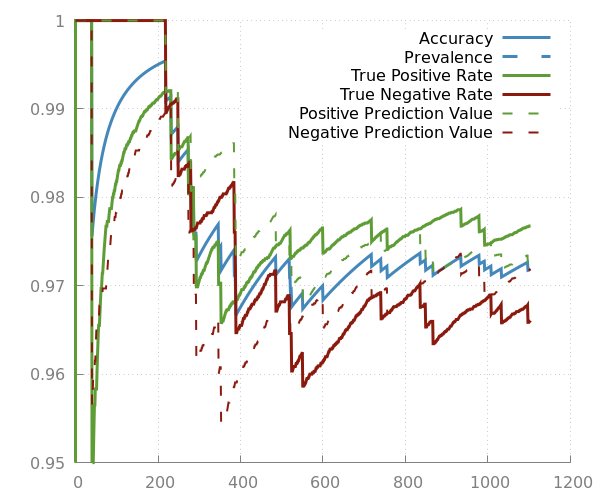
\includegraphics[scale=0.35]{img/output_run_0_confusion_matrix_1.png}
\caption{Evolution of the confusion matrix during the prediction phase for \texttt{phishing} dataset.}
\label{fig:evolution_phishing}
\end{figure}
The average confusion matrix obtained for each dataset is showed in Table \ref{table:confusion_matrix}. The performance indicators are reported in Table \ref{table:perf_indicators}. The proposed algorithm performs very well on a wide range of datasets as reported by \cref{table:confusion_matrix,table:perf_indicators}, in particular when they contain strong predictors as it is the case for \texttt{mushroom}. The accuracy is contained in a range from 0.8206 (\texttt{adult}) to 1 (\texttt{mushrooms}) while the $F_1$-score is bounded by 0.8653 (\texttt{heart}) and 1 (\texttt{mushrooms}). On \texttt{adult}, the accuracy is only 6\% higher than the prevalence. A model consisting in returning 1 for any point would be only 6\% worse. This relatively poor performance in learning the underlying decision mapping is better reflected by the Matthews correlation coefficient of $0.51$.

The false positives and false negatives are equilibrated for each dataset, despite a huge variation in the prevalence (between 20\% and 64\%, cf. Table \ref{table:confusion_matrix}) which may be a desirable property depending on applications. In addition, the results were obtained with non-balanced training sets which are known to be a problem for many machine learning algorithms. Moreover, the performance indicators remain stable during the whole prediction phase as shown on Figure \ref{fig:evolution_phishing} for the dataset \texttt{phishing} (similar result is observed for all datasets).

For a given case, the support is a metric of confidence in the prediction as illustrated in Figure \ref{fig:phishing_predictive_measure}. In general, the wrongly classified cases have a smaller difference between the evidence for each class which confirm the interest in the hyperparameters $\eta$ and $\bar \eta$ used in \eqref{eqn:updated_cr}.

\begin{figure}[!h]
\centering
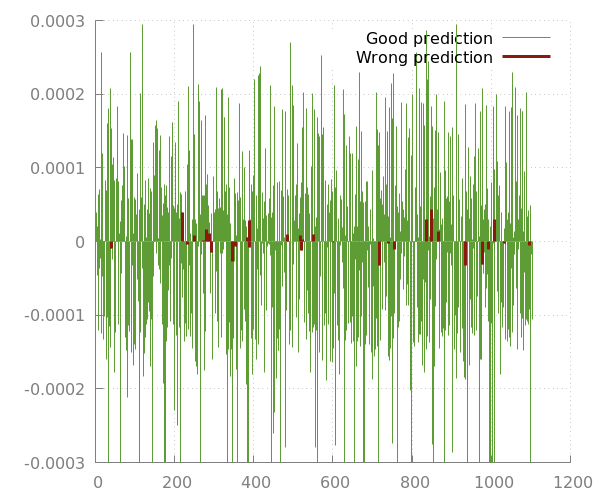
\includegraphics[scale=0.35]{img/output_run_0_diff_pred_1.png}
\caption{Difference between the weight assigned to both classes for each decision on \texttt{phishing} (average). Similar results are observed for all datasets.}
\label{fig:phishing_predictive_measure}
\end{figure}

To compare the results of the proposed method, we explored the best results from the literature for each dataset. The comparison with \texttt{audiology} is not relevant due to the transformation into a two-class problem. The results are summarized in Table \ref{table:prev_results}. In \cite{doi:10.1504/IJBISE.2016.081590}, 5 rule-based classification techniques dedicated to medical databases are compared and achieve at best 95.85\% and 82.96\% accuracy resp. on \texttt{breast}, and \texttt{heart} datasets. Comparing bayesian approaches, \cite{Jiang:2012:LIW:2124637.2124641} demonstrated 97.35\% (\texttt{breast}) and 83.00\% (\texttt{heart}) accuracy. A 5 layers neural network with fuzzy inference rules achieved 87.78\% on \texttt{heart} \cite{sagir2017hybridised} while a k-NN algorithm reached 99.96\% on \texttt{mushrooms} \cite{Das:2001:FWB:645530.658297}. The best alternative among 6 rules-based classification methods achieved 95.84\% on \texttt{breast} and 100.00\% on \texttt{mushroom} \cite{HADI2017287}. Using 80\% of \texttt{phishing} as training set, an adaptative neural network achieved an average accuracy of 93.76\% (among 6 alternatives) with the best run at 94.90\% \cite{7727750}. Still on \texttt{phishing}, \cite{7881507} proposes to combine several classifiers and reaches 97.75\% accuracy for the best hybrid model (and demonstrates 97.58\% for Random Forest classifier). On \texttt{adult}, the comparison of several classifiers (naive bayes, decision tree, ...) demonstrated at most 86.25\% accuracy \cite{kou2012evaluation} while a Support Vector Machine approach reached 85.35\% \cite{Lee2001}. On \texttt{splice}, a method using Fuzzy Decision Trees \cite{5409447} reaches 94.10\% accuracy and a neural network combined to boosting \cite{catak2017} 97.54\%. On \texttt{breast}, Support Vector Machine approaches reached resp. 96.87\%, 98.53\%, 99.51\% accuracy \cite{CHEN20119014, POLAT2007694, akay2009support}, 99.26\% and 97.36\% for neural network based techniques \cite{MARCANOCEDENO20119573, ubeyli2007implementing}, 98.1\% for a bayesian network method \cite{fallahi2011expert}, or 94.74\% using Decision Trees \cite{quinlan1996improved}. On \texttt{skin}, \cite{catak2017} reports 98.94\% accuracy against 99.68\% for Decision Tree based method~\cite{6627823}. The best result, as far as we know, is 99.92\%, obtained by a Generalized Linear Model~\cite{basterrech2015generalized} (with 80\% training set).

The accuracy is slightly lower than the best results from the literature (\texttt{adult} 82.06\% against 86.25\%, \texttt{breast} 96.96\% against 99.51\%, \texttt{heart} 85.77\% against 87.78\%, \texttt{phishing} 96.05\% against 97.75\%, \texttt{splice} 94.43\% against 97.54\%, \texttt{skin} 98.65\% against 99.92\%). We explain this by at least two factors. First, the best methods on a given dataset are often dedicated to this dataset with {\it ad-hoc} or engineered parts which is not the case of \HCBR. Secondly, the hyperparameter familly $\eta$ have not been tuned but as we will show in next section, they might have a decisive impact on performance.
\HCBR~ performed better than Bayes classifier in two thirds of cases. Bayes classifier performs better on \texttt{breast} by \~1\% which represents less than one case wrongly classified. Similar results are observed with Decision Trees. However, the 1\% difference on \texttt{skin} represents an average of 7 cases misclassified in comparison in favor of Bayes. It performs better than Rule-based approaches (or gives similar results on \texttt{mushrooms} with an accuracy of 1) in the four considered references on three different datasets. Notice that combined with Neural Network, Rule-based achieves the state-of-art result on \texttt{heart} dataset. Except for \texttt{phishing}, Neural Network returns better results ($0.46$ more cases with correct classification in average for \texttt{breast}, $71$ for skin and almost $10$ for \texttt{splice}). Last, SVM gives better results in all three cases, but appear only as best results in two datasets.
\begin{table}[htbp]
\begin{center}
  \caption{Average confusion matrix obtained with a 10-fold cross-validation.}
 %\resizebox{12cm}{!}{
  \begin{small}
  \begin{tabular}{|l|c|c|c|c|c|c|c|c|c|c|c|}
    \hline
     & TP & FN & FP & TP & Prevalence\\
    \hline
    \texttt{adult} & 2182.40 & 295.30 & 288.50 & 488.80 & 0.7586\\
    \texttt{audiology} & 12.70 & 0.10 & 0.00 & 6.20 & 0.6048\\
    \texttt{breast} & 23.00 & 1.40 & 0.70 & 43.90 & 0.3338\\
    \texttt{heart} & 12.40 & 1.80 & 1.90 & 9.90 & 0.5107\\
    \texttt{mushrooms} & 390.60 & 0.00 & 0.00 & 420.40 & 0.4804\\
    \texttt{phishing} & 595.40 & 23.80 & 19.80 & 465.00 & 0.5562\\
    \texttt{skin} & 4886.30 & 132.40 & 199.40 & 19286.90 & 0.2075\\
    \texttt{splice} & 155.70 & 9.10 & 8.50 & 142.70 & 0.5164\\
    \hline
  \end{tabular}
  \end{small}
  %}
  \label{table:confusion_matrix}
\end{center}
\end{table}
\begin{table*}[htbp]
\begin{center}
  \caption{Average performances obtained with a 10-fold cross-validation.}
 %\resizebox{12cm}{!}{
  \begin{small}
  \begin{tabular}{|l|c|c|c|c|c|c|c|c|c|c|c|}
    \hline
     & Accuracy (standard dev.) & Recall & Specificity & Precision & Neg. Pred. Value & $F_1$ score & Matthews corr. coef.\\
    \hline
    \texttt{adult} & 0.8206 (0.0094) & 0.8832 & 0.6233 & 0.8808 & 0.6290 & 0.8820 & 0.5081\\
    \texttt{audiology} & 0.9947 (0.0166) & 1.0000 & 0.9875 & 0.9917 & 1.0000 & 0.9957 & 0.9896\\
    \texttt{breasts} & 0.9696 (0.0345) & 0.9691 & 0.9676 & 0.9479 & 0.9844 & 0.9575 & 0.9344\\
    \texttt{heart} & 0.8577 (0.0943) & 0.8695 & 0.8437 & 0.8699 & 0.8531 & 0.8653 & 0.7178\\
    \texttt{mushrooms} & 1.0000 (0.0000) & 1.0000 & 1.0000 & 1.0000 & 1.0000 & 1.0000 & 1.0000\\
    \texttt{phishing} & 0.9605 (0.0081) & 0.9680 & 0.9514  & 0.9615 & 0.9590 & 0.9647 & 0.9199\\
    \texttt{skin} & 0.9865 (0.0069) & 0.9608 & 0.9932  &0.9736 & 0.9898 & 0.9672 & 0.9587 \\
    \texttt{splice} & 0.9443 (0.0124) & 0.9478 & 0.9398 & 0.9450 & 0.9441 & 0.9463 & 0.8884\\
    \hline
  \end{tabular}
  \end{small}
  %}
  \label{table:perf_indicators}
\end{center}
\end{table*}
\begin{table}[tb]
\begin{center}
  \caption{Previous literature results measured as the highest accuracy obtained by the authors.}
  %\resizebox{12cm}{!}{
  \begin{small}
\begin{tabular}{|c|c|l|c|}
\hline
 Dataset & Ref. & Type & Accuracy   \\ \hline
\multirow{2}{*}{\texttt{adult}} & \cite{kou2012evaluation} & Many classifiers &  86.25\% \\
& \cite{Lee2001} & SVM & 85.35\% \\ 
& & \bfHCBR & {\bf 82.06\%} \\ \hline
 \multirow{10}{*}{\texttt{breast}} & \cite{akay2009support}  & SVM & 99.51\% \\ 
 & \cite{MARCANOCEDENO20119573} & Neural Network & 99.26\% \\ 
 & \cite{POLAT2007694} & SVM & 98.53\% \\ 
 & \cite{fallahi2011expert} & Bayes & 98.1\% \\ 
 & \cite{ubeyli2007implementing} & Neural Network & 97.36\% \\ 
 & \cite{Jiang:2012:LIW:2124637.2124641} & Bayes & 97.35\% \\ 
 & & {\bf \bfHCBR} & {\bf 96.96\%} \\
 & \cite{CHEN20119014} & SVM & 96.87\% \\
 & \cite{doi:10.1504/IJBISE.2016.081590} & Rule-based & 95.85\% \\
 & \cite{HADI2017287} & Rule-based & 95.84\% \\
 & \cite{quinlan1996improved} & Decision Tree & 94.74\% \\ \hline
 \multirow{3}{*}{\texttt{heart}} & \cite{sagir2017hybridised} & Neural Network + Rule-based & 87.78\%\\
 & & {\bf \bfHCBR} & {\bf 85.77\%} \\
 & \cite{Jiang:2012:LIW:2124637.2124641} & Bayes & 83.00\% \\ 
 & \cite{doi:10.1504/IJBISE.2016.081590} & Rule-based & 82.96\% \\ \hline
 \multirow{2}{*}{\texttt{mushrooms}} &  \cite{HADI2017287} & Rule-Based & 100.00\% \\ 
  & & {\bf \bfHCBR} & {\bf 100.00\%} \\
  & \cite{Das:2001:FWB:645530.658297} & k-NN & 99.96\% \\ \hline
 \multirow{3}{*}{\texttt{phishing}} & \cite{7881507} & Ensemble & 97.75\% \\ 
 &  \cite{7881507} & Random-Forest & 97.58\% \\ 
 & & {\bf \bfHCBR}& {\bf  96.05\%} \\
 & \cite{7727750} & Neural Network &  94.90\% \\\hline
 \multirow{3}{*}{\texttt{skin}} & \cite{basterrech2015generalized} & Generalized Linear Model & 99.92\% \\ 
 & \cite{6627823} & Decision Tree & 99.68\% \\ 
 & \cite{catak2017} & Neural Network + Boosting & 98.94\% \\
 & & {\bf \bfHCBR} & {\bf 98.65\%} \\ \hline
 \multirow{2}{*}{\texttt{splice}} & \cite{catak2017} & Neural Network + Boosting & 97.54\% \\
 & & {\bf \bfHCBR} & {\bf 94.43\%} \\
 & \cite{5409447} & (fuzzy) Decision Tree & 94.10\% \\ \hline
\end{tabular}
\end{small}
  %}
  \label{table:prev_results}
\end{center}
\end{table}
\subsection{Intrinsic performance}

In this section, we evaluate the capacity of \HCBR~ to build an efficient model (w.r.t. the accuracy measure) with few examples. We also study the influence of the two main parameters (number of examples and size of the examples) on the computation time.\\

\noindent
{\bf Training set size:} To evaluate \HCBR, we used a standard 90-10 dataset split in the previous section. Additionally, we studied the accuracy depending on the split from 1\% to 99\%. For each split value, we performed 100 runs with random splits and averaged the accuracy. As shown in Figure \ref{fig:accuracy}, \HCBR~ reaches its maximal accuracy with about 15\% of the dataset as examples. The dataset \texttt{adult} shows a constant results from 1\% while for \texttt{audiology} more than 40\% is required to achieve over 90\% accuracy. Despite the datasets having different sizes (e.g. \texttt{skin} is 350 larger than \texttt{breast}), the trajectories look the same. Further work should focus on determining the optimal training set size depending on the size of cases and the underlying measure to generate them in $\mathcal P({\mathbb F})$ (as it influences the induced hypergraph, it influences the strength measure and thus the decisions). Additional experiments need to be performed to fairly compare those results to the existing algorithms. However, it is commonly accepted that non-linear classifiers requires very large training sets.\\
\begin{figure}[!h]
\centering
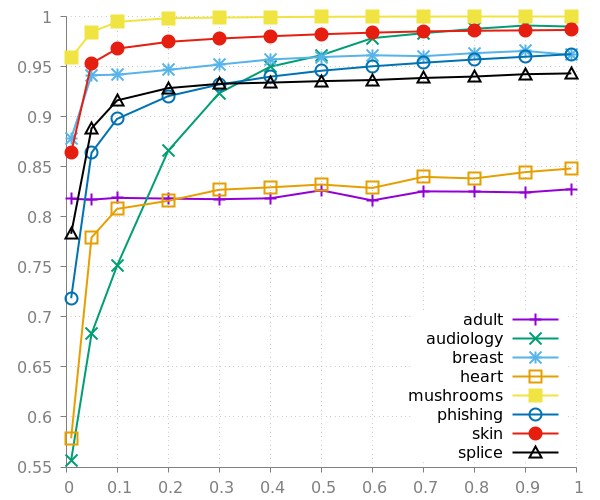
\includegraphics[scale=0.35]{img/accuracy_by_examples.png}
\caption{Accuracy depending on the percentage of the dataset used as training set.}
\label{fig:accuracy}
\end{figure}

%\newpage
\noindent
{\bf Computation Time:} We generated a casebase of $n$ cases of size $m$ such that case $i$ is described by $\{i, ...,  i+m\}$ i.e., each case is partitioned into $m$ elements (one discretionary feature). This is the worst-case scenario in terms of the size of $\mathcal{E}$ if $m < n$ because the family grows exponentially in function of $m$ or $n$. We split the computation time into constructing the hypergraph (and determining the intersection family) and calculating the strength of the partition. The results are illustrated in Figure \ref{fig:time}. By increasing $n$ with a fixed $m$, the partition grows exponentially and thus, it is expected to have an exponential curve for the strength computation. On the contrary, building the hypergraph can be done in linear time when $m$ fixed. When $n$ is fixed and $m$ increases, constructing the hypergraph is still doable in linear time as expected. Interestingly, calculating the strength has two phases: if $m \leq n$, increasing $m$ exponentially increases the time (because $\mathcal{E}$ exponentially increases) but if $m > n$, increasing $m$ cannot results in an exponential growth in the computation time (because $\mathcal{E}$ grows linearly).

\begin{figure}[!h]
\centering
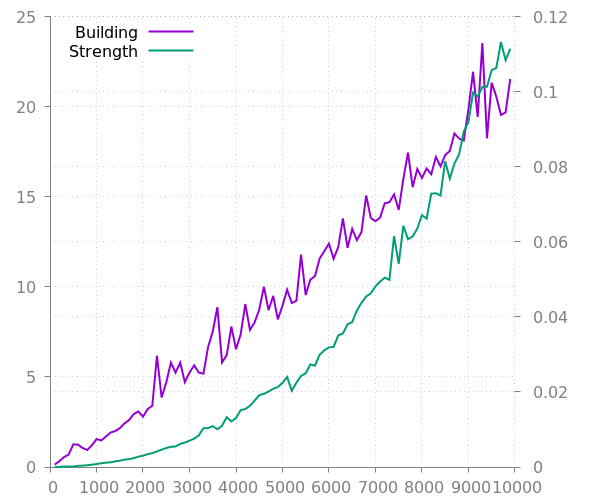
\includegraphics[scale=0.35]{img/time_k.png}
\hfill
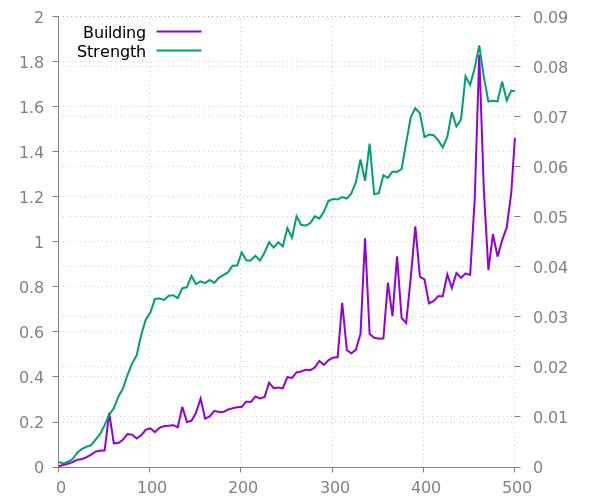
\includegraphics[scale=0.35]{img/time_n_old.png}
\caption{At the top, computation time to build the model (hypergraph construction + strength calculation) depending on $n$ ($m = 10$), and at the bottom, depending on $m$ ($n = 100$). The case $i$ is described by $\{i, ...,  i+m\}$ such that each case is partitionned into $m$ elements (one discretionary feature). Right scale for bulding and left scale for strength.}
\label{fig:time}
\end{figure}

~\\\noindent
{\bf Hyperparameters $\eta$:} We used a 90-10 split and set $\eta_0 = \eta_1$ to ease the visualization. Instead of using the decision function defined by \eqref{eqn:decision_rule_revised}, we did not produce a prediction if the constraints $C_1$ or $C_0$ were not respected. It can be viewed as creating a third class {\it unknown} for which we consider we cannot produce a decision. We measured the accuracy and the test set size ratio for which a prediction has been produced for different values of $\eta := \eta_0 = \eta_1$. If $\bar J$ correctly approximates $J$, increasing $\eta$ should increase the accuracy while the test set ratio should remain high. Additionally, we plot the test set ratio in function of the accuracy and calculate the Pareto frontier\footnote{Points such that improving one component would degrades the other one.} which represents the best compromises accuracy/ratio. The closer the points are to $(1,1)$ the better it is. A Pareto frontier consisting of $(1,1)$ represents the perfect model (e.g. reached on \texttt{mushroom} dataset). Figures \ref{fig:meta_phishing}, \ref{fig:meta_breast}, \ref{fig:meta_heart} and \ref{fig:meta_adult} provides the result for the best and worst two datasets. Figure \ref{fig:meta_all} shows all of the four Pareto frontiers. 
\begin{figure}[!h]
\centering
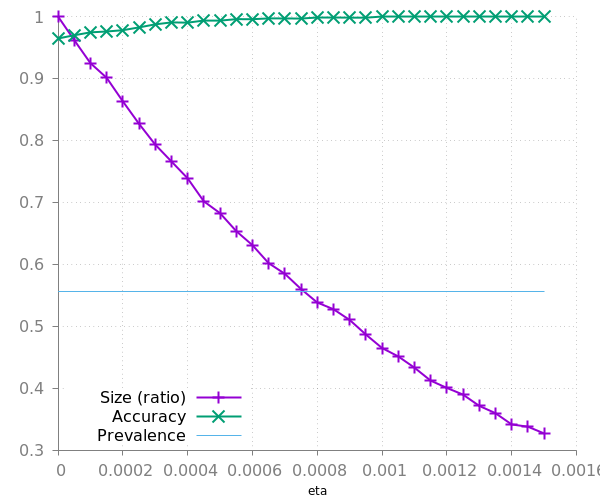
\includegraphics[scale=0.35]{img/meta_phishing.png}
\hfill
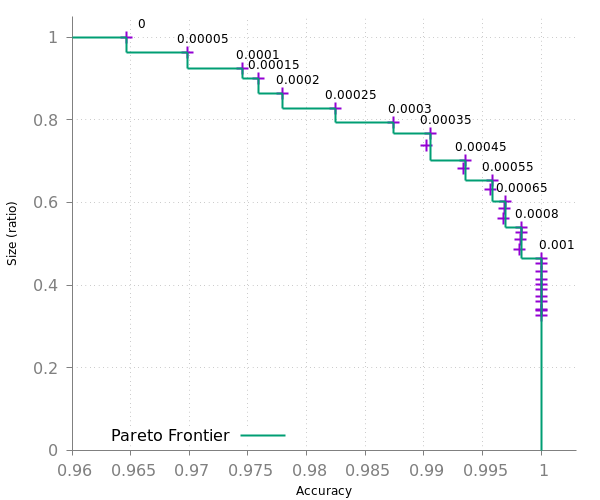
\includegraphics[scale=0.35]{img/meta_pareto_phishing.png}
\caption{Influence of $\eta$ on \texttt{phishing} dataset.}
\label{fig:meta_phishing}
\end{figure}
As expected, the results are better on \texttt{phishing} and \texttt{breast}. On \texttt{phishing}, \texttt{breast} and \texttt{heart}, the accuracy globally increases with $\eta$ while on \texttt{heart} the accuracy slightly decreases indicating poor influence of the hyperparameters and model. 

Notice that for certain values of $\eta$ it is possible to reach 100\% accuracy with \texttt{heart} while it is not with \texttt{breast}. Also, for high values of $\eta$, we observe a fall in accuracy for \texttt{breast}. We suspect those two phenomena to appear because we used the same value for $\eta_0$ and $\eta_1$. 

\begin{figure}[!h]\centering
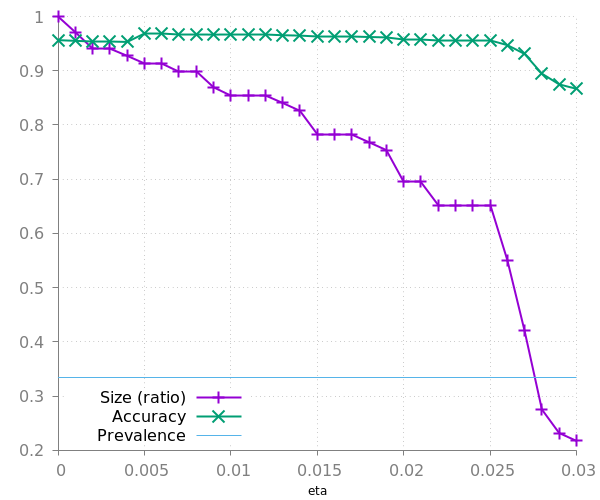
\includegraphics[scale=0.35]{img/meta_breast.png}
\hfill
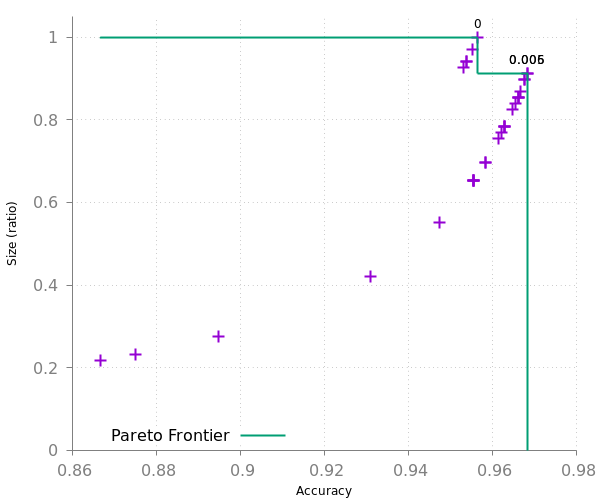
\includegraphics[scale=0.35]{img/meta_pareto_breast.png}
\caption{Influence of $\eta$ on \texttt{breast} dataset.}
\label{fig:meta_breast}
\end{figure}
\begin{figure}[!h]
\centering
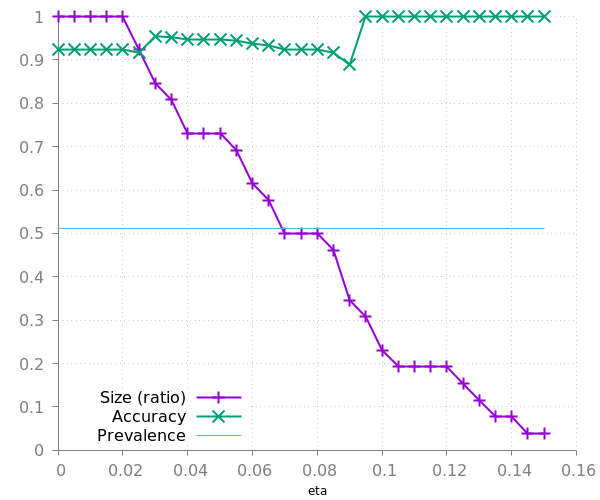
\includegraphics[scale=0.35]{img/meta_heart.png}
\hfill
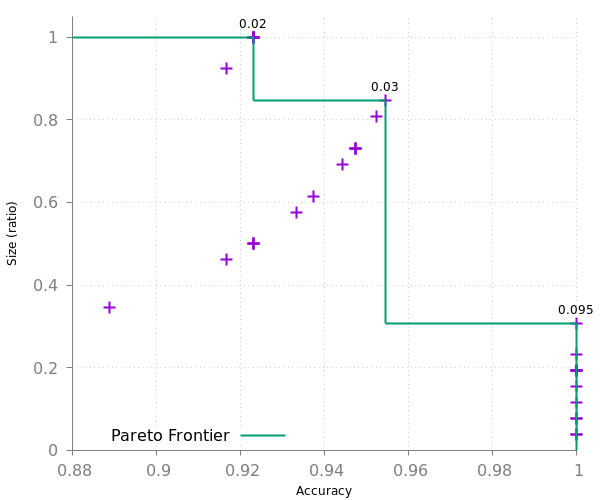
\includegraphics[scale=0.35]{img/meta_pareto_heart.png}
\caption{Influence of $\eta$ on \texttt{heart} dataset.}
\label{fig:meta_heart}
\end{figure}
\begin{figure}[!h]\centering
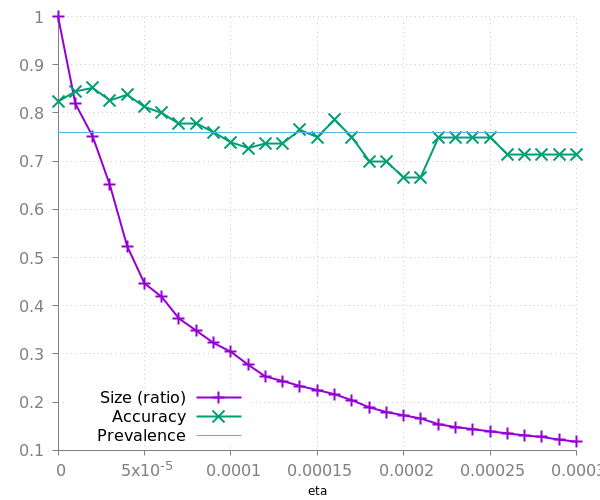
\includegraphics[scale=0.35]{img/meta_adult.png}
\hfill
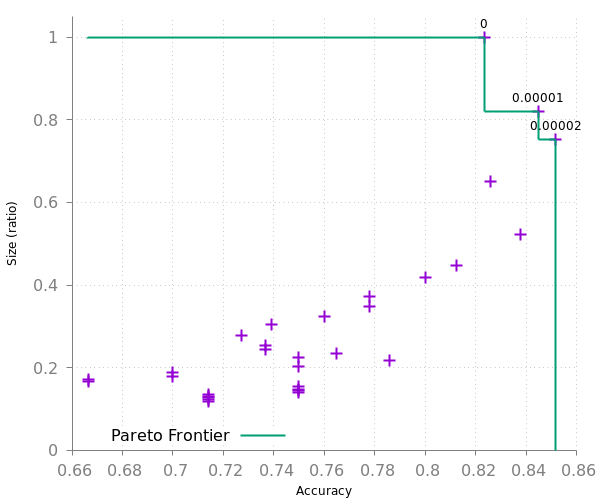
\includegraphics[scale=0.35]{img/meta_pareto_adult.png}
\caption{Influence of $\eta$ on \texttt{adult} dataset.}
\label{fig:meta_adult}
\end{figure}
More work is required to fully study the influence of the hyperparameters $(\eta_0, \eta_1, \bar \eta_0, \bar \eta_1)$ and how to select $l_0$ and $l_1$. We believe it is the key to improve the overall performance, and it is possible to derivate the best values from the training set. Also, a comparison with binary classification methods that provide a prediction confidence metric is necessary.
\begin{figure}[!h]\centering
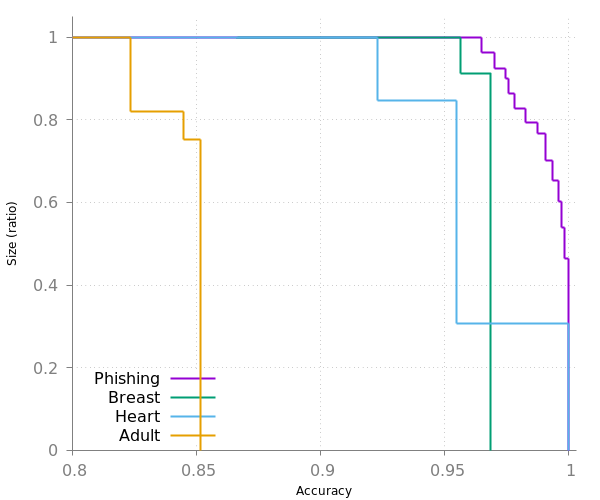
\includegraphics[scale=0.35]{img/meta_pareto_all_front.png}
\caption{Pareto Frontiers comparison.}
\label{fig:meta_all}
\end{figure}

%\newpage
\section{Conclusion}
\label{sec:conclusion}

This paper presented \HCBR, a method for binary classification using a hypergraph representation of information and building a convex combination out of the induced partition to determine the support for each class. The general framework introduced by \eqref{eqn:model} is instantiated in Section \ref{sec:model_selection} where the support is determined using all the interactions between the hyperedges. Beyond this specific implementation, one can imagine different model selection methods to be used, e.g. using some assumptions on the data.

However, being totally agnostic on the data representation is convenient compared to many methods such as SVM. It allows combining information from multiple sources by simply {\it stacking} the information. It does not require transforming the data to fit the algorithm, often by designing specific ad-hoc metrics.

\HCBR~ has been tested on 8 well-known datasets and demonstrated similar accuracies when compared to the best results from the literature. The algorithm has shown a strong stability in terms of accuracy, true positive and negative rates during the whole prediction phase. We showed that the difference of class support is a good confidence indicator for the prediction. We demonstrated the capacity to obtain a good accuracy using very few examples from the dataset (10\% to 15\% of the training set) without balanced classes. This last property is very important for robustness as in practice, the dataset are rarely balanced. Finally, we empirically validated the exponential worst-case complexity.

This proof of concept raises many questions and offer many improvement axes. First of all, it seems relatively easy to extend the method to several classes but it needs an additional empirical validation. As most of the computational effort is on calculating the class support, adding more classes will linearly increase the computation time and thus, working on a faster algorithm or an approximation of the main measure should be investigated. The solution may come from exploring the feature selection capacity of \HCBR. Indeed, by the hypergraph construction, it may be possible to remove from the partition some elements that do not participate enough (e.g. not being in enough cases at the same time), reducing the computation time.
Additionally, we plan to investigate how to generate an explanation about each prediction and one about the decision function $J$ itself, using not only the convex combination and the strength of the partition elements, but also the link between cases in a similar way a lawyer may use past cases to make analogies or counter-examples. We also work on an online version of \HCBR~ where the hypergraph is constructed case after case, including forgetting some old past cases (which would allow handling non-stationary environment). It seems also possible not only to add new examples dynamically, but also some vertices (i.e. adding some pertinent information to some cases) without generating the whole model from scratch. 

Empirically, further experiments should focus on more unstructured datasets (for instance for text classification). As stated previously, strategies for hyperparameter tunning are also a priority.
Last but not least, we would like to answer some questions: is it possible to find a method to adjust the strength measure such that the accuracy on the training set is 1? Can we provide some quality bounds depending on the initial hypergraph and thus the dataset? How to handle continuous values?

\section*{Acknowledgment}

The author warmly thanks Pr. Robert Wrembel, Poznan University of Technology, and Dr. Jean-Fran\c{c}ois Puget, IBM Analytics, for their useful suggestions and advice to improve this paper.

\bibliographystyle{ACM-Reference-Format}
\bibliography{paper} 

\end{document}